\section{Approach and Uniqueness\label{sec:approach}}
\begin{figure}
    \begin{center}
        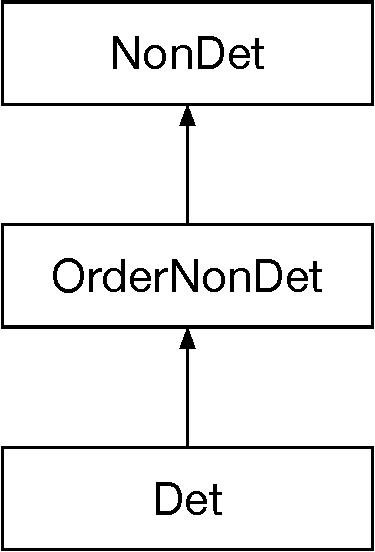
\includegraphics[scale=0.37]{detHierarchy}
    \end{center}
    \caption{Determinism type qualifier hierarchy}
    \label{fig:determinism-hierarchy}
\end{figure}

The most novel part of our analysis is how it handles collections that will
contain the same values, but
possibly in a different order, on different runs.

The core of the determinism type system\todo{This is the first mention of
  the determinism type system, and the first mention of types since the
  abstract.  This is sudden and unexpected, and it will confuse readers.
  You need to say that you will take this approach to solving the problem!}
is the following type qualifiers:\todo{The introduction of the type
  qualifiers is too sudden, too.  What are type qualifiers?  How are they
  used?  Why does a reader care?  You should say that every expression in
  the program is classified as one of the following categories.}
\begin{itemize}
    \item \<NonDet> indicates
    that the expression might have different values in two different executions.
    \item \<OrderNonDet> indicates that the expression is a collection or
    a map that contains the same elements in every execution, but possibly
    in a different order.
    \item \<Det> indicates that the expression evaluates to equal values in
    all executions; for a collection, iteration
    also yields the values in the same order.
\end{itemize}
\Cref{fig:determinism-hierarchy} shows the subtyping
relationship among the qualifiers.
Programmers can write these type qualifiers to specify their program's behavior.
\todo{Cut the following sentence, which uses jargon like ``basetype'' that
  has not been defined, and therefore is offputting and confusing to readers.}The basetypes of their elements can be specified independently of the collection basetypes.
\todo{For the following sentence, show an example, or give the typing rule,
  or both.}However, an element type qualifier must be a subtype of the collection type qualifier.
\OurTypeSystem checks all the standard typing rules\todo{``all the standard
  typing rules'' is too glib.  It denigrates the reader by implying that
  the reader ought to know this already, or that the paper is intended only
  for a narrow audience with a specific technical background.  Make the
  paper more welcoming.  Give a couple examples, and maybe even show source
  code for them.}
of an object-oriented programming language where the types have these
additional type qualifiers.
\todo{The following three things are the same.  Why are they listed as
  different?  Also, their purpose is to reduce false positive warnings,
  rather than to enable better reporting of true positives.  Also, try to
  explain terms when you introduce them.  If you don't have space for that,
  then ask yourself if this point is important enough to include in the paper.}It performs dataflow analysis,
type refinement and local type inference to precisely report specification violations.

\subsubsection{Behavior of order-nondeterministic collections}\label{sec:ond-behavior}
A collection of type \<OrderNonDet> has special properties that are enforced by additional typing rules in \ourTypeSystem.
\todo{Like other parts of the document (and as noted by the referees), this
  feels vague.  Make it more concrete, with examples or with specific explanation.}

\begin{enumerate}
    \item
    The individual elements retrieved from it have type \<NonDet>.  This
    affects access, iteration, searching, etc.
    \item
    Size-related operations return a deterministic result.  This affects
    queries of whether an iterator has more elements.
    \item
    If the collection is sorted, or its elements are placed in a collection
    that does sorting, the result is deterministic.
\end{enumerate}

%%  LocalWords:  NonDet OrderNonDet Det basetype offputting basetypes
